\section{Jealousy}

\begin{center}
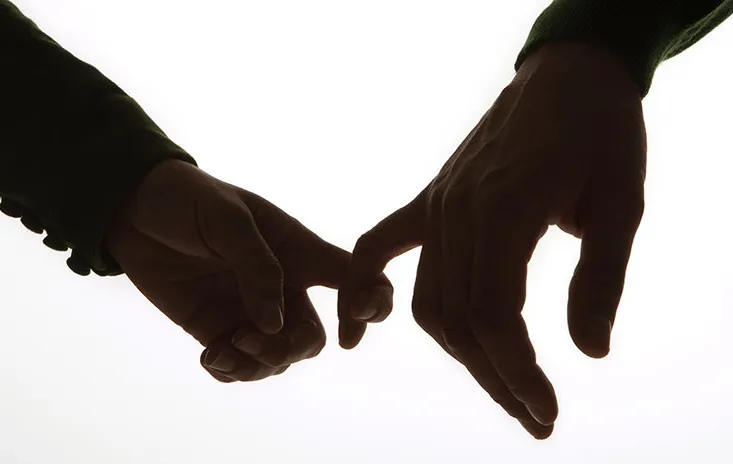
\includegraphics[width=7cm]{images/12_jealousy.png}
\end{center}

\textit{Believing that jealousy has something to do with love is a misconception.}

"The more you love someone, the more jealously you react", "Jealousy is proof of love" - we have been hearing such statements ever since we were kids: Cheap novels want to convince us and pop songs drool those kind of lyrics upon us.

Truth be told, it is more like this seemingly superficial German saying states: "\textit{Eifersucht ist eine Leidenschaft, die mit Eifer sucht, was Leiden schafft}" (jealousy is a passion, which seeks with eagerness, what creates suffering). Take, for example, when we justbroke up with our partner, and that partner then gets engaged with another person. Or: It doesn't seem like a big thing for you to have a side-relationship, but if your partner claims to have the same right, you get indignant.

In the name of love, which is supposedly the source of jealousy, we beat others verbally and physically. When one suffers, the other will be made to suffer too. Threats, blackmailing, torture and homicide can follow. There are still countries where the so-called "murder out of passion" is still free of persecution (of course only for men). Does this look like love?

When we have a close look at the impactful effects of jealousy, we quickly can identify its roots: Violence has two main sources: the claim to power and fear. (Even if violence is expressed very mildly through punishment by sulking or dramatically by making a scene, threats or physical violence, or even against the one who is jealous himself, reaching from "I haven't deserved it any better" to suicide).The power claim is based on the conviction that one has the right to decide over the lifestyle of the other, or at least have a big influence on it. This self-proclaimed right is based on the belief that the other person "belongs to oneself".

Today we are all too well educated to speak out such things loudly. However, the imprints of past centuries and millennia still have a relentless, hidden influence on us. We feel those painfully when we get in contact with geographically more remote cultural conceptions, that are getting more tangible now.

There is this fear to lose that power, on the one hand, and to be not good enough on the other.  The fear of competing, of getting uncomfortable, of letting go of safety and of confronting oneself with a novel situation. Of being forced to let go of territory, or of consenting to new, less comforting agreements for the ego.

The combination of a claim to power and fear is highly explosive, and shows itself on the surface as anger and revenge ("\textit{What?! You hurt me?! Just wait, I'll show you!}") or also as victimization ("\textit{I will never be able to trust someone again}") and leads to those kind of discharges which are well known in scenes of jealousy.

In order to throw a devastating punch at our former beloved one and now deadly enemy, no big words are necessary, as often a small glance is sufficient to destroy what has been built up over a long period of time. So what do we do in such a specific case, so that the jealousy bomb won't blow up?

\begin{enumerate}
\item First of all, you have to admit that you are jealous, because the ego likes to conceal it behind justified anger, fake indifference,...
\item Furthermore, you have to be clear that jealousy doesn't lead to any constructive results for anyone: It can only destroy, persistently.
\item Next step: Try to reason what's behind the jealousy. Do I identify myself through my partner and am I scared to disappear once my partner is not there anymore for me? Am I outraged because someone entered my territory? Do I feel insecure because the other one is younger, knows better how to deal with computers, ...? Do I actually want to hide and cry, because I am panicking over change?
\item Communication. Very often, being jealous lacks any real foundation (this also relates to the German saying at the beginning of this chapter): Maybe the other person was her cousin? Maybe she just enjoyed the flirtatious eye contact with the waiter because he made her feel reassured about  her femininity -and that's it?
\item Tell the other person what's happening inside of you. Start the sentence with "I ...", as in: "I am terribly mad because I have the feeling that ...", or "I am totally insecure because ...", or "I have a problem with ...". Avoid generalizations like: \textit{ever, never, always, a hundred times}.
\item If it is impossible to talk about this topic without overwhelming emotions, ask a person whom you both trust to join you. Just their presence can smoothen the emotional waves. It is a sign of maturity to ask for professional help when in need.
\item And yet again: Talk with each other!
\item If that is currently not possible at all: Be silent with each other. Keep eye contact for about 20 minutes and let the eyes do the talk.
\item Let the bodies also do the talking. The body often wants something totally different than the scared heart or the confused head. Touching each other’s hands and communicating with the fingertips can be a stunning and utterly reconciling experience.
\item If there has not happened anything seriously bad yet, and the deeply injured ego can let it happen: Sleep with each other. In case your despite is insurmountable, be aware that you don't deceive yourself. From a certain perspective, you are not surrendering to your partner, but always to love itself, your own love!
\end{enumerate}

A sexual encounter, which is rooted in love and happens for that love, and that is not abused to pressure someone, is a powerful medicine and can lead you two to the point where you both know what you mean to each other. Regardless of how strong the wind howls outside.
